\documentclass{standalone}
\usepackage{tikz}
\usepackage{tkz-euclide}
\usepackage{ctex}
\setCJKmainfont{Noto Serif CJK SC}
\usepackage{mhchem,siunitx}
\begin{document}
\small
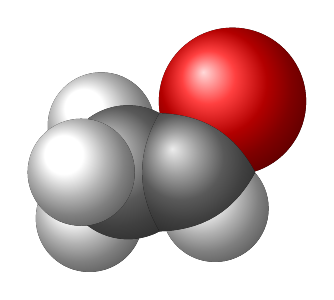
\begin{tikzpicture}[scale=1.7]
  \fill[ball color=white](120:0.4)circle(0.4);
  \fill[ball color=white](230:0.45)circle(0.4);
  \fill[ball color=white](0.65,-0.27)circle(0.4);
  \fill[ball color=gray](0,0)circle(0.5);
  \fill[ball color=white](-0.35,0)circle(0.4);
  \fill[ball color=red](0.78,0.53)circle(0.55);
  \fill[ball color=gray](62:0.5)to[bend right](-62:0.5)to[bend right](0.95,0)to[bend right]cycle;
\end{tikzpicture}
\end{document}